\section{การดำเนินการสร้างและติดตั้งระบบ (Implementation)}
\label{sec:implementation}

\subsection{การประกอบเชิงกล (Mechanical Assembly)}
\label{sec:mech_assembly}

\subsubsection{ภาพรวมการประกอบ (Overview)}
\label{sec:mech_overview}
หัวข้อนี้อธิบายถึงภาพรวมและขั้นตอนการประกอบชิ้นส่วนทางกลของหุ่นยนต์ โดยมีองค์ประกอบและเครื่องมือที่จำเป็นต้องใช้ในการประกอบ ดังแสดงในรูปที่ \ref{fig:exploded_iso} และ \ref{fig:exploded_side}

ชิ้นส่วนหลักประกอบด้วย ส่วนฐาน (Base), ส่วนแขนกลและมอเตอร์ (Arm \& Motor), ชุดมือจับ (Gripper), ชุดเอ็นโค้ดเดอร์ (Encoder), สายพาน (Belt), คัปปลิ้ง (Coupling) และเพลาเชื่อมต่อเอ็นโค้ดเดอร์สนาม (Field Encoder Shaft) สำหรับเครื่องมือที่ใช้ในการประกอบ ได้แก่ ประแจหกเหลี่ยม ประแจปากตาย ประแจแหวน และค้อน

\begin{figure}[H]
  \centering
  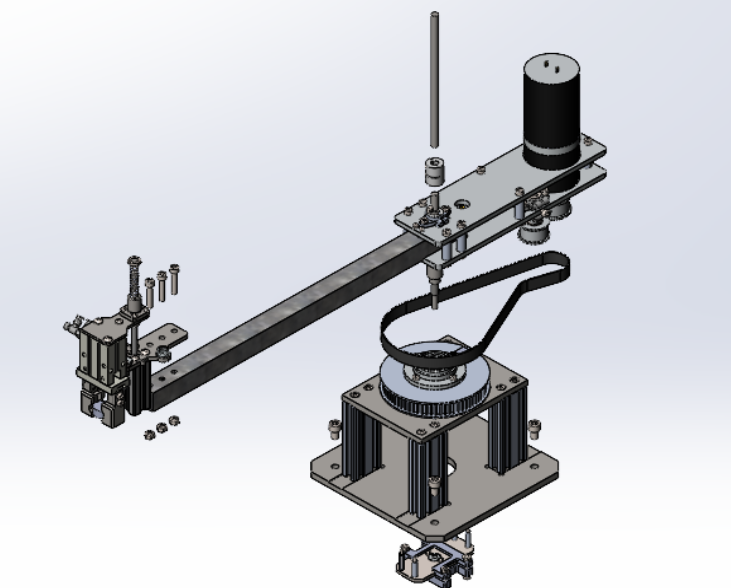
\includegraphics[width=0.88\textwidth]{images/Explode_ISO.png}
  \caption{ภาพรวมชิ้นส่วนของหุ่นยนต์ (Exploded View) ในมุม Isometric}
  \label{fig:exploded_iso}
\end{figure}

\begin{figure}[H]
  \centering
  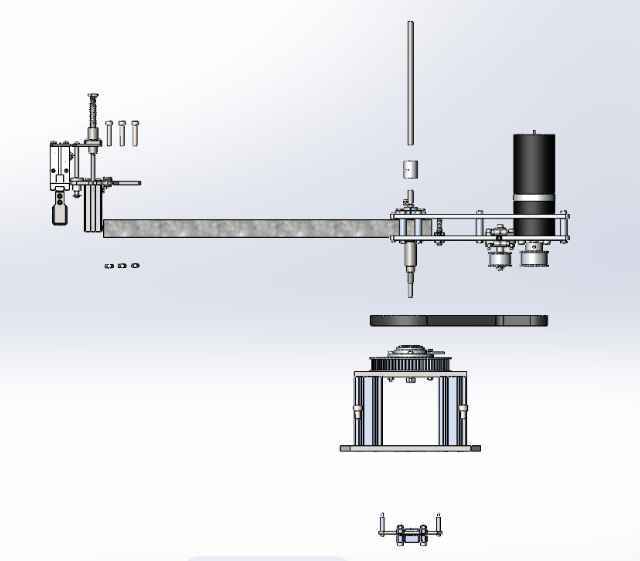
\includegraphics[width=0.88\textwidth]{images/Explode_side.png}
  \caption{ภาพรวมชิ้นส่วนของหุ่นยนต์ (Exploded View) ในมุม Side View}
  \label{fig:exploded_side}
\end{figure}

\subsubsection{ขั้นตอนการประกอบชิ้นส่วนย่อย (Sub-assembly Process)}
\label{sec:sub_assembly}
การประกอบชิ้นส่วนทางกลจะเริ่มจากการประกอบชิ้นส่วนย่อย (Sub-assemblies) 3 ส่วนหลัก เพื่อให้ง่ายต่อการตรวจสอบและลดข้อผิดพลาด ดังนี้

\paragraph{1. ส่วนฐาน (Base Sub-assembly)}
\label{sec:base_assembly}
รายการชิ้นส่วนที่ใช้ในการประกอบส่วนฐานแสดงไว้ในตารางที่ \ref{tab:base_parts}

\begin{table}[H]
\centering
\caption{รายการชิ้นส่วนสำหรับประกอบส่วนฐาน (Base Sub-assembly)}
\label{tab:base_parts}
\begin{tabular}{llc}
\toprule
ชิ้นส่วน & รายละเอียด & จำนวน \\
\midrule
อลูมิเนียมโปรไฟล์ 20x40 & ยาว 100 mm & 4 \\
แผ่นชิ้นฐานหุ่น (Base Plate) & ทำจาก AISI 316 & 1 \\
แผ่นชิ้นรอง Pulley & ทำจาก AISI 316 & 1 \\
Pulley & 72 ฟัน ID 19 mm & 1 \\
Bearing Mounting & ทำจากเหล็ก & 1 \\
Tapered Roller Bearing & ID 17 mm, OD 40 mm & 1 \\
ชิ้นส่วน Set Home & ทำจากเหล็ก & 1 \\
Ball Bearing & ID 12 mm, OD 19 mm & 1 \\
Socket Head Cap Screw M5 & ยาว 12 mm & 16 \\
Socket Head Cap Screw M4 & ยาว 40 mm & 4 \\
Nut M4 & - & 4 \\
\bottomrule
\end{tabular}
\end{table}

ขั้นตอนการประกอบส่วนฐานมีดังนี้
\begin{enumerate}
    \item \textbf{การประกอบโครงสร้างฐาน (Base):} นำอลูมิเนียมโปรไฟล์ $20\times40$ ทั้ง 4 ชิ้น มาประกอบเข้ากับแผ่นชิ้นฐานหุ่น (Base Plate) โดยจัดวางให้อลูมิเนียมโปรไฟล์สวมลงในร่องของแผ่นฐานพอดี จากนั้นใช้สกรู M5 ยาว 12 mm จำนวน 8 ตัว ขันยึดให้โครงสร้างตั้งฉากและแน่นหนา
    \item \textbf{การติดตั้งแผ่นรอง (Pulley Mounting Plate):} นำแผ่นชิ้นรอง Pulley มาประกอบปิดทับอลูมิเนียมโปรไฟล์ $20\times40$ จากทางด้านบน โดยจัดให้รูน็อตของอลูมิเนียมโปรไฟล์และแผ่นชิ้นรองตรงกัน แล้วใช้สกรู M5 ยาว 12 mm จำนวน 8 ตัว ขันยึดให้โครงสร้างทั้งหมดตั้งฉากและแน่นหนา
    \item \textbf{การวางพูลเลย์ (Pulley Placement):} วาง Pulley 72 ฟัน (ID 19 mm) ลงในตำแหน่งแกนกลางของแผ่นชิ้นรอง Pulley โดยหมุนจัดให้รูน็อตของทั้งสองชิ้นอยู่ในตำแหน่งที่ตรงกัน
    \item \textbf{การยึดเสื้อลูกปืน (Bearing Mounting):} นำ Bearing Mounting วางลงไปที่ตำแหน่งแกนกลางของ Pulley และจัดรูน็อตให้ตรงกัน จากนั้นยึดชิ้นส่วนทั้งหมดเข้ากับโครงสร้างฐานด้วยสกรู M4 ยาว 40 mm จำนวน 3 ตัว แล้วขันล็อกด้วยน็อตตัวเมีย (Nut) ให้แน่น
    \item \textbf{การติดตั้งตลับลูกปืน (Bearing Installation):} ใส่ตลับลูกปืนเม็ดเรียว (Tapered Roller Bearing) สวมเข้าไปด้านบนของ Bearing Mounting และนำตลับลูกปืนเม็ดกลม (Ball Bearing) ใส่เข้าไปที่รูแกนกลางบริเวณใต้แผ่นชิ้นรอง Pulley
    \item \textbf{การติดตั้งชิ้นส่วนอ้างอิง (Set Home):} นำชิ้นส่วน Set Home มาประกอบเข้ากับ Bearing Mounting บริเวณรูน็อตที่ยังว่างอยู่ จากนั้นใช้สกรู M4 ยาว 40 mm ยึดชิ้นส่วน Set Home เข้ากับ Bearing Mounting แล้วขันล็อกให้แน่นด้วยน็อตตัวเมีย (Nut)
\end{enumerate}

\paragraph{2. ส่วนแขนกลและข้อต่อ (Arm Links \& Joints)}
\label{sec:arm_assembly}
รายการชิ้นส่วนที่ใช้ในการประกอบส่วนแขนกลแสดงไว้ในตารางที่ \ref{tab:arm_parts}

\begin{table}[H]
\centering
\caption{รายการชิ้นส่วนสำหรับประกอบส่วนแขนกลและข้อต่อ}
\label{tab:arm_parts}
\begin{tabular}{llc}
\toprule
ชิ้นส่วน & รายละเอียด & จำนวน \\
\midrule
Motor & - & 1 \\
แผ่นชิ้นส่วนแขนกล (บน) & ทำจาก Aluminum Alloy 6061 & 1 \\
แผ่นชิ้นส่วนแขนกล (ล่าง) & ทำจาก Aluminum Alloy 6061 & 1 \\
เหล็กกล่อง Galvanized & ขนาด 25x25 mm & 1 \\
Stepped Shaft & ทำจาก Stainless Steel & 1 \\
Pulley & 20 ฟัน ID 12 mm & 1 \\
Idler & ID 10 mm, Width 15 mm & 1 \\
Shaft Support & 10 mm Aluminum Alloy & 3 \\
บูชรอง & M5 OD 10x57 mm & 1 \\
บูชรอง & M6 OD 8x2 mm & 4 \\
บูชรอง & M5 OD 10x25 mm & 8 \\
Key (ลิ่ม) & ขนาด 5x5x8 mm & 1 \\
Proximity Sensor & ขนาด 12 mm & 1 \\
สกรูและน็อตต่างๆ & สกรู M3, M5, M6 และน็อตกันคลาย & 33 \\
\bottomrule
\end{tabular}
\end{table}

ขั้นตอนการประกอบส่วนแขนกลมีดังนี้
\begin{enumerate}
    \item นำแผ่นชิ้นส่วนแขนกลบนและล่าง มาประกบเข้ากับเหล็กกล่อง Galvanized โดยใช้บูชรอง (M5 OD 10x25 mm) เพื่อรักษาระยะห่าง และใช้บูชรอง (M6 OD 8x2 mm) เพื่ออุดพื้นที่ว่างบริเวณด้านบนเหล็กกล่อง Galvanized จากนั้นร้อยสกรู M5 แล้วขันล็อกด้วยน็อต (Nut M5) ให้แน่น
    \item ติดตั้งมอเตอร์เข้ากับแผ่นแขนกล จากนั้นสวม Pulley 20 ฟัน เข้ากับเพลามอเตอร์
    \item สอด Stepped Shaft เข้ากับจุดหมุนหลักของแขน โดยใส่ Key (ลิ่ม 5x5x8) เพื่อป้องกันการหมุนฟรีของเพลา จากนั้นติดตั้ง Shaft Support เพื่อประคองแกนเพลาให้มั่นคง
    \item ติดตั้งลูกกลิ้งประคองสายพาน (Idler) ด้วยบูชรองและสกรูที่กำหนด พร้อมทั้งติดตั้ง Proximity Sensor สำหรับใช้เป็นเซนเซอร์อ้างอิงตำแหน่ง (Limit/Homing)
    \item ตรวจเช็คการประกอบโดยขันน็อตทุกจุดให้แน่นตามค่าแรงบิด (Torque) ที่เหมาะสม และตรวจสอบการเคลื่อนที่ของข้อต่อ
\end{enumerate}

\paragraph{3. ส่วนชุดเอ็นโค้ดเดอร์ (Encoder Sub-assembly)}
\label{sec:encoder_assembly}

\begin{table}[H]
\centering
\caption{รายการชิ้นส่วนสำหรับประกอบชุดเอ็นโค้ดเดอร์}
\label{tab:encoder_parts}
\begin{tabular}{llc}
\toprule
ชิ้นส่วน & รายละเอียด & จำนวน \\
\midrule
บูชรอง & M3 OD 5.5x20 mm & 4 \\
AMT Mounting & ทำจาก AISI 316 & 1 \\
Encoder & รุ่น AMT-103 & 1 \\
ชิ้นส่วนประกบ Encoder (บน/ล่าง) & ทำจาก 3D Print & อย่างละ 1 \\
สกรูและน็อต & M2 4mm, M3 30mm, M5 25mm & 16 \\
\bottomrule
\end{tabular}
\end{table}

ขั้นตอนการประกอบชุดเอ็นโค้ดเดอร์มีดังนี้
\begin{enumerate}
    \item \textbf{การติดตั้งเซนเซอร์ (Encoder Installation):} นำ Encoder รุ่น AMT-103 มาติดตั้งลงบนแผ่นยึด AMT Mounting โดยใช้สกรู M2 ยาว 4 mm ขันยึดให้เข้าตำแหน่ง จากนั้นขันล็อกด้วยน็อตตัวเมีย (Nut M2) ให้แน่น
    \item \textbf{การประกอบชิ้นส่วนรองรับ (Bottom Enclosure):} นำชิ้นส่วนประกบ Encoder แบบ 3D Print (ด้านล่าง) มาวางรองรับตัวเอ็นโค้ดเดอร์ จากนั้นสอดสกรู M5 เข้าที่รูน็อตทั้ง 4 จุด
    \item \textbf{การปิดฝาครอบ (Top Enclosure):} นำชิ้นส่วนประกบ 3D Print (ด้านบน) มาครอบปิดทับ สอดสกรู M5 ผ่านรูร้อยของชิ้นส่วนประกบทั้งสองฝั่ง และขันล็อกด้วยน็อตตัวเมีย (Nut M5) ที่ด้านล่างให้แน่นหนา
    \item \textbf{การติดตั้งเข้ากับส่วนฐาน (Base Mounting):} นำชุดเอ็นโค้ดเดอร์มาเตรียมติดตั้งเข้ากับฐาน โดยใส่บูชรองขนาด M3 เข้าที่ตำแหน่งรูน็อตทั้ง 4 จุดเพื่อรักษาระยะช่องว่าง (Clearance) จากนั้นใช้สกรู M3 ยาว 25 mm จำนวน 4 ตัวยึดชุดเอ็นโค้ดเดอร์เข้ากับส่วนฐาน
\end{enumerate}

\subsubsection{ลำดับขั้นตอนการประกอบรวม (Final Assembly Process)}
\label{sec:final_assembly}
หลังจากประกอบชิ้นส่วนย่อยเสร็จสิ้น ให้ดำเนินการประกอบรวมเป็นหุ่นยนต์เต็มรูปแบบตามลำดับดังต่อไปนี้
\begin{enumerate}
    \item \textbf{การติดตั้งเอ็นโค้ดเดอร์เข้ากับฐาน:} นำชุดเอ็นโค้ดเดอร์ไปประกอบเข้ากับส่วนฐาน โดยขันน็อตยึดเข้ากับรูต๊าปเกลียวบนฐานให้แน่นหนา
    \item \textbf{การใส่สายพาน:} นำชุดฐานที่ยึดเข้ากับเอ็นโค้ดเดอร์แล้ว มาทำการคล้องสายพาน (Belt) เตรียมไว้สำหรับการส่งกำลัง
    \item \textbf{การประกอบแขนกลและมอเตอร์:} นำส่วนแขนกลและมอเตอร์มาประกอบเข้ากับฐาน โดยสอดเพลาของส่วนแขนกลลงไปในรูร้อยแกนกลางของส่วนฐาน
    \item \textbf{การตั้งค่าพรีโหลดตลับลูกปืน (Bearing Preload):} จัดวางให้ส่วนแขนกลและมอเตอร์กดทับลงบนตลับลูกปืนเม็ดเรียว (Tapered Roller Bearing) ของส่วนฐาน จากนั้นทำการขันน็อตที่เพลาเพื่อเป็นการให้แรงดึงล่วงหน้า (Preload) แก่ตลับลูกปืนเม็ดเรียว ซึ่งจะช่วยลดระยะคลอนของกลไก
    \item \textbf{การเชื่อมต่อเอ็นโค้ดเดอร์สนาม:} นำเพลาเชื่อมต่อเอ็นโค้ดเดอร์สนามมาต่อเข้ากับเพลาบริเวณด้านบนสุดของหุ่นยนต์ โดยใช้คัปปลิ้ง (Rigid/Flexible Shaft Coupling) เพื่อให้เอ็นโค้ดเดอร์สามารถอ่านตำแหน่งการหมุนของเพลาได้อย่างแม่นยำ
    \item \textbf{การติดตั้งชุดมือจับ (Gripper):} นำชุดมือจับประกอบเข้ากับปลายแขนของหุ่นยนต์ ทำการยึดด้วยน็อตจำนวน 3 ตัว และขันล็อกให้แน่นหนาด้วยน็อตกันคลาย (Lock Nut)
\end{enumerate}

\subsection{การจัดระเบียบสายไฟและระบบไฟฟ้า (Cable Management)}
\label{sec:cable_management}
การจัดระเบียบสายไฟ (Cable Management) ถือเป็นขั้นตอนสำคัญเพื่อให้หุ่นยนต์ทำงานได้อย่างเสถียรและปลอดภัย โดยมีแนวทางปฏิบัติดังนี้
\begin{itemize}
    \item \textbf{การเผื่อระยะสายบริเวณจุดหมุน (Service Loop):} บริเวณข้อต่อของแขนกล (Joints) จะต้องมีการเผื่อความยาวของสายไฟ (Slack) ให้หย่อนในระดับที่เหมาะสม เพื่อให้สายไฟสามารถโค้งงอได้อย่างอิสระเมื่อหุ่นยนต์เคลื่อนที่ไปจนถึงระยะสูงสุด (Maximum Reach) การเผื่อระยะนี้จะช่วยป้องกันปัญหาสายไฟดึงรั้ง ขาดใน หรือขั้วหลุด
    \item \textbf{การควบคุมรัศมีการโค้งงอ (Bending Radius):} มีการติดตั้งชิ้นส่วน 3D Print ที่มุมของหุ่นยนต์ เพื่อบังคับให้มีรัศมีการโค้งงอของสายไฟที่เพียงพอ ป้องกันไม่ให้สายไฟหักมุมแคบเกินไป ซึ่งเป็นการรักษาสภาพของสายสัญญาณภายใน
\end{itemize}

% ============================================================
% เพิ่มใน Section 3.1 ต่อจาก subsubsection{ลำดับขั้นตอนการประกอบ}
% ============================================================

\subsubsection{แบบวิศวกรรม (Engineering Drawing)}
\label{subsubsec:engineering_drawing}


% [รูป Engineering Drawing 2D Top/Front/Side]
% \begin{figure}[H]
%   \centering
%   \includegraphics[width=0.95\textwidth]{images/engineering_drawing.png}
%   \caption{Engineering Drawing แสดง Top View,
%            Front View และ Side View
%            พร้อมมิติสำคัญ}
%   \label{fig:engineering_drawing}
% \end{figure}

% รูปที่~\ref{fig:engineering_drawing} แสดง
% Engineering Drawing พร้อมมิติที่สำคัญ
% สำหรับการผลิตและประกอบ

รายละเอียด Drawing แต่ละชิ้นส่วนแสดงใน Appendix A

\subsubsection{ปัญหาและการแก้ไขที่พบระหว่างการประกอบ}
\label{subsubsec:assembly_issues}

ระหว่างการประกอบพบปัญหาเชิงกลหลายประการดังนี้

\begin{itemize}
  \item \textbf{รู Proximity Sensor}: ขนาดรูที่ออกแบบไว้คือ
        $\diameter$8\,mm แต่ขนาด Sensor จริงต้องการ $\diameter$12\,mm
        จึงต้องเจาะขยายรูเพิ่มในภายหลัง
  \item \textbf{รู Driver Pulley และ Arm เบี้ยว}:
        ชิ้นส่วนที่ส่งไปผลิตที่ร้านภายนอกมีรูไม่ตรงแนวศูนย์
        เนื่องจากการ Setup งานของร้านผู้ผลิตไม่ตรงกับแบบ
        แก้ไขโดยนำกลับไปปรับแต่งเพิ่มเติม
  \item \textbf{ชิ้นแผ่นรอง Pulley}: ร้านผู้ผลิตไม่ได้ปาดผิวหน้า
        ชิ้นงานให้ราบเรียบตามแบบ และไม่ได้ร่อง Aluminium Profile
        ให้ตามที่กำหนด จึงต้องดำเนินการแก้ไขเพิ่มเติมเองใน Lab
  \item \textbf{ปัญหา Shaft Tolerance และ Bearing Housing Tolerance:} 
      ในชิ้นส่วน Shaft และ Bearing Housing มี Tolerance ที่ขนาดใหญ่มากเกินไปทำให้ไม่สามารถใส่ได้พอดี ทำให้ต้องเอาไปเข้าเครื่องกลึงแล้วเอากระดาษทรายขัดออกจนทำให้สามารถใส่อัดได้ด้วยมือ แต่เมื่อแก้แล้วทำให้ fit น้อยกว่าที่ตั้งใจไว้แต่แรก
  \item \textbf{ความยาวสายพานที่ซื้อมานั้นมีขนาดสั้นกว่าที่วางแผนไว้:} 
      ทำให้ต้องมีการปรับขนาดความยาวชิ้นส่วน 2 ส่วน เพื่อไว้สามารถทำให้สายพานตึงได้ตามที่ออกแบบไว้เมื่อใช้ร่วมกับ Tensioner Pulley ตามที่ออกแบบไว้
  \item \textbf{มีการเจาะรูน็อตที่คลาดเคลื่อนที่ Pulley:} 
      ทำให้ต้องไปเจาะเพิ่มในแนวใหม่ทั้ง 4 รู
\end{itemize}

% ----------------------------------------------------------------------------
% 3.2.3 สรุปความคลาดเคลื่อนของชิ้นงานเทียบกับ Drawing และแนวทางการแก้ไข
% ----------------------------------------------------------------------------
\subsubsection{สรุปความคลาดเคลื่อนของชิ้นงานเทียบกับ Drawing และแนวทางการแก้ไข}
\label{subsubsec:part_discrepancy_summary}

จากการตรวจสอบชิ้นงานจริง พบว่ามีชิ้นงานจำนวน 5 รายการ ที่มีข้อกำหนดคลาดเคลื่อนไปจากแบบวิศวกรรมหลายจุด ทางทีมงานจึงได้ทำการรวบรวม วิเคราะห์สาเหตุ และกำหนดแนวทางแก้ไข ดังรายละเอียดต่อไปนี้

\paragraph{3.2.3.1 ตารางสรุปภาพรวมชิ้นงานที่พบปัญหา (Master Summary of Discrepancies)}
\label{par:master_summary_discrepancies}

\begin{table}[H]
    \centering
    \caption{ตารางสรุปภาพรวมชิ้นงานที่พบปัญหา}
    \label{tab:discrepancy_summary}
    \begin{tabular}{clcp{7cm}}
        \toprule
        \textbf{ลำดับ} & \textbf{ชื่อชิ้นงาน (Part Name)} & \textbf{จำนวนจุดที่พบปัญหา} & \textbf{สถานะการจัดการเบื้องต้น} \\
        \midrule
        1 & Body Plate & 2 จุด & มีการเปลี่ยนขนาดน็อตที่ใช้กับจุดที่มีปัญหา และมีการเจาะขยายรูในจุดที่มีปัญหาอีกจุด \\
        2 & TOP Plate & 1 จุด & มีการเขียน Drawing ขนาดรูผิดทำให้ต้องขยายขนาดรูเพิ่ม \\
        3 & Bearing Mounting & 1 จุด & ต้องนำเข้าเครื่องกลึงแล้วใช้กระดาษทรายขัดเพื่อปรับขนาด tolerance ให้สามารถใส่ Bearing Case ได้ \\
        4 & Arm & 2 จุด & มีรูน็อตที่เจาะเบี้ยวทำให้ต้องขยายรูเพิ่มเพื่อให้สามารถประกอบร่วมกับชิ้นงานอื่นได้ \\
        5 & Platev & 1 จุด & มีจุดที่ต้องปาดออกแต่โดยรวมยังประกอบได้จึงยังไม่ได้แก้ไข \\
        \bottomrule
    \end{tabular}
\end{table}

\paragraph{3.2.3.2 สรุปสาเหตุร่วมของระบบและแนวทางแก้ไขภาพรวม (Systemic Issues \& Corrective Actions)}
\label{par:systemic_issues_corrective_actions}

จากการวิเคราะห์ปัญหาความคลาดเคลื่อนที่เกิดขึ้นในหลาย Drawing ซึ่งเป็นชิ้นงานที่สั่งผลิตจากร้านภายนอก (Supplier) ด้วยกระบวนการตัดด้วยเลเซอร์ (Laser Cutting) พบว่ามี ``สาเหตุร่วม (Common Causes)'' ดังต่อไปนี้:

\textbf{สาเหตุร่วมของความคลาดเคลื่อน:}
\begin{enumerate}
    \item \textbf{การตั้งค่าชดเชยรอยตัดเลเซอร์ (Laser Kerf / Beam Offset):} ทางร้านภายนอกอาจมีการตั้งค่าเผื่อระยะความกว้างของลำแสงเลเซอร์ในโปรแกรมตัด (CAD/CAM) ไม่พอดีกับความหนา หรือชนิดของวัสดุ ทำให้ขนาดจริงคลาดเคลื่อนไปจากแบบเล็กน้อย
    \item \textbf{ข้อจำกัดด้านพิกัดความเผื่อของเครื่องจักร (Machine Tolerance):} ความคลาดเคลื่อนเล็กน้อยที่เกิดขึ้น อาจอยู่ในช่วงพิกัดความคลาดเคลื่อนมาตรฐานของเครื่องตัดเลเซอร์ที่ทางร้านใช้งานอยู่ (ซึ่งอาจกว้างกว่าที่ระบุไว้ใน Drawing)
    \item \textbf{การสื่อสารเรื่องพิกัดความเผื่อ (Tolerance Communication):} แบบ Drawing อาจกำหนดค่าพิกัดความเผื่อที่แคบเกินไป (Tight Tolerance) สำหรับงานตัดเลเซอร์ทั่วไป โดยไม่ได้ตกลงรายละเอียดกับร้านภายนอกให้ชัดเจนก่อนเริ่มงาน
\end{enumerate}

\textbf{แผนการแก้ไขภาพรวมและการจัดการร้านภายนอก (Overall Action Plan \& Supplier Management):}
\begin{itemize}
    \item \textbf{การจัดการชิ้นงานล็อตปัจจุบัน (Disposition):} เนื่องจากเป็นความคลาดเคลื่อนเพียงเล็กน้อย ทำให้สามารถยอมรับชิ้นงาน (Concession / Accept as is) เพื่อนำไปใช้งานได้เลย หากทดลองประกอบแล้วไม่ส่งผลกระทบต่อการทำงาน (Functional Impact) เพื่อให้งานเดินหน้าต่อได้
    \item \textbf{การสื่อสารและปรับปรุงร่วมกับร้านภายนอก (Supplier Feedback):} จัดส่งรายงานแจ้งผลการตรวจสอบ (Inspection Report) ให้ทางร้านรับทราบถึงจุดที่ขนาดคลาดเคลื่อน เพื่อให้ทางร้านปรับตั้งค่าชดเชยรอยตัด (Offset) ใหม่สำหรับการสั่งผลิตในล็อตถัดไป
    \item \textbf{การทบทวนแบบวิศวกรรม (Drawing Review):} ฝ่ายออกแบบควรพิจารณาปรับแก้พิกัดความเผื่อ (Tolerance) ใน Drawing ให้เหมาะสมและสอดคล้องกับธรรมชาติของงานตัดเลเซอร์มากขึ้น หากจุดนั้นๆ ไม่ได้ซีเรียสเรื่องความแม่นยำสูง เพื่อลดปัญหาการตีงานเสีย (Reject) โดยไม่จำเป็น
\end{itemize}

% ------------------------------------------------------------
\subsection{การประกอบตู้ควบคุมไฟฟ้า (Electrical Cabinet Assembly)}
\label{subsec:electrical_cabinet_assembly}
% ------------------------------------------------------------

\subsubsection{รายการอุปกรณ์ภายในตู้}
\label{subsubsec:cabinet_equipment_list}

\begin{table}[H]
  \centering
  \caption{Bill of Materials (BOM) ของตู้ควบคุม}
  \label{tab:bom}
  \begin{tabular}{llcc}
    \toprule
    Reference & อุปกรณ์ & จำนวน & หมายเหตุ \\
    \midrule
    U1A       & STM32G474RE Nucleo Board    & 1 & Main Controller \\
    U2        & ESP32-DEVKIT-V1             & 1 & Joystick Receiver \\
    --        & Cytron MD10C Motor Driver   & 1 & 24V/10A \\
    CB1       & Circuit Breaker 10A         & 1 & AC Input Protection \\
    CB2       & Circuit Breaker 5A          & 1 & 24V Bus Protection \\
    CB3       & Circuit Breaker 3A          & 1 & 5V Bus Protection \\
    --        & PSU 24V/10A                 & 1 & Motor Power \\
    --        & PSU 5V/5A                   & 1 & Logic Power \\
    --        & Step-down Converter 12V     & 1 & Auxiliary \\
    --        & Magnetic Contactor          & 1 & E-Stop Interlock \\
    --        & Optocoupler Module 8-ch     & 1 & Signal Isolation \\
    --        & Relay Module 4-ch           & 1 & Output Control \\
    --        & Emergency Stop Button       & 1 & NC Contact \\
    --        & Pilot Lamp Blue (Power)     & 1 & Power Status \\
    --        & Pilot Lamp Red (Emergency)  & 1 & Fault Status \\
    --        & Pilot Lamp Green (Ready)    & 1 & Ready Status \\
    --        & Reset Button                & 1 & NC Contact \\
    --        & Mode Selector Switch        & 1 & Manual/Auto \\
    --        & Fuse (Motor Circuit)        & 1 & Short Circuit Protection \\
    \bottomrule
  \end{tabular}
\end{table}

\subsubsection{ผลการประกอบตู้ควบคุม}
\label{subsubsec:cabinet_assembly_result}

% [รูปที่ XX: ผลการเดินสายภายในตู้ควบคุมไฟฟ้า]
% \begin{figure}[H]
%   \centering
%   \includegraphics[width=0.78\textwidth]{images/cabinet_assembled.png}
%   \caption{ผลการเดินสายภายในตู้ควบคุมไฟฟ้า}
%   \label{fig:cabinet_assembled}
% \end{figure}

การเดินสายภายในตู้ควบคุมแบ่งออกเป็น 2 วงจรหลัก
ที่แยกจากกันอย่างชัดเจนตามที่ออกแบบไว้ใน Section~2.2
สัญญาณดิจิทัลทุกเส้นที่เชื่อมระหว่าง High Voltage Side
และ Logic Side ผ่าน Optocoupler Module
เพื่อแยก Ground และป้องกัน Noise จากมอเตอร์

% ------------------------------------------------------------
\subsection{สถาปัตยกรรม STM32 Firmware (Firmware Architecture)}
\label{subsec:firmware_architecture}
% ------------------------------------------------------------

\subsubsection{ภาพรวมสถาปัตยกรรม Firmware}
\label{subsubsec:firmware_architecture_overview}

Firmware พัฒนาบน STM32CubeIDE โดยใช้ HAL Library
แบ่งออกเป็น 3 โมดูลหลักที่สื่อสารกันผ่าน Interrupt
และ Shared Variable ดังแสดงในตารางที่~\ref{tab:firmware_modules}

\subsubsection{โครงสร้างไฟล์และโมดูล (Code Structure)}
\label{subsubsec:code_structure}

\begin{table}[H]
  \centering
  \caption{โมดูลหลักใน STM32 Firmware}
  \label{tab:firmware_modules}
  \begin{tabular}{lp{7cm}l}
    \toprule
    โมดูล & หน้าที่ & ไฟล์ \\
    \midrule
    \texttt{motor\_controller} &
      Encoder อ่านค่าตำแหน่งและความเร็ว,
      Cascade PID (Position + Speed Loop),
      S-Curve Trajectory Generator,
      Joystick Command Parser,
      Safety Monitor (Stall, Encoder Fault,
      Over-Rotation, E-Stop) &
      \texttt{motor\_controller.c} \\
    \addlinespace
    \texttt{modbus\_bridge} &
      Modbus Register Mapping (128 registers),
      Command Dispatch จาก Master,
      Status Update ไปยัง Register Frame &
      \texttt{modbus\_bridge.c} \\
    \addlinespace
    \texttt{modbus\_rtu} &
      Modbus RTU Protocol Engine,
      CRC16 Verification,
      Frame Parser (FC03, FC06),
      State Machine (IDLE/RECEPTION/
      PROCESSING/EMISSION) &
      \texttt{modbus\_rtu.c} \\
    \addlinespace
    \texttt{main} &
      Peripheral Initialization,
      Callback Registration,
      Main Loop (Modbus Process,
      Register Update, MATLAB Data Send) &
      \texttt{main.c} \\
    \bottomrule
  \end{tabular}
\end{table}

\subsubsection{Interrupt Service Routine (ISR) และ Timing}
\label{subsubsec:isr_and_timing}

\begin{table}[H]
  \centering
  \caption{ISR และ Task Timing ของ Firmware}
  \label{tab:isr_timing}
  \begin{tabular}{lllll}
    \toprule
    Timer/Peripheral & โหมด & Period & หน้าที่ & Callback \\
    \midrule
    TIM6  & Base, IT   & 10\,ms (100\,Hz) &
      Control Loop (\texttt{Motor\_ControlLoop}) &
      \texttt{Timer\_PeriodElapsedCallback} \\
    TIM16 & Base, IT   & 3\,ms &
      Modbus T3.5 Timeout &
      \texttt{Timer\_PeriodElapsedCallback} \\
    TIM3  & Encoder QEI & -- &
      Quadrature Encoder Count (TIM\_ENCODERMODE\_TI12) &
      -- (Polling ใน Control Loop) \\
    TIM8  & PWM CH2    & $f_{PWM}$ = \(170\,\text{MHz} / (170 \times 51)\) $\approx$ 19.6\,kHz &
      Motor PWM Output &
      -- \\
    LPUART1 & UART RX IT & -- &
      Modbus RTU Byte Reception &
      \texttt{Modbus\_RxCallback} \\
    USART3  & UART RX IT & -- &
      Joystick Command Reception (115200\,8N1) &
      \texttt{Joystick\_RxCallback} \\
    \bottomrule
  \end{tabular}
\end{table}

หมายเหตุ: TIM6 ตั้งค่า Prescaler = 169, Period = 9999
ที่ System Clock 170\,MHz ได้ Period จริง
$= (169+1)(9999+1)/170\,\text{MHz} = 10\,\text{ms}$
ดังนั้น Control Loop Rate = 100\,Hz
และ \texttt{control\_dt} = 0.01\,s

\subsubsection{การทำงานร่วมกันของโมดูล (Module Interaction)}
\label{subsubsec:module_interaction}

การทำงานของ Firmware แบ่งออกเป็น 2 Context ดังนี้

\textbf{Interrupt Context} (Priority สูง):
\texttt{Modbus\_RxCallback} รับ Byte ทีละตัวจาก LPUART1
แล้วเก็บใน RX Buffer และ Reset T3.5 Timer
\texttt{Joystick\_RxCallback} รับ Command Character
จาก USART3 แล้วเรียก \texttt{Motor\_ProcessCommand}
ทันที และ \texttt{Timer\_PeriodElapsedCallback} ของ TIM6
เรียก \texttt{Motor\_ControlLoop} ทุก 10\,ms

\textbf{Main Loop Context} (Priority ต่ำ):
\texttt{ModbusBridge\_UpdateRegisters} ซิงค์ค่าตำแหน่ง
และความเร็วปัจจุบันลง Register Frame,
\texttt{ModbusBridge\_Process} รัน Protocol Engine
และ Dispatch คำสั่งจาก Master และ
\texttt{Motor\_SendDataToMatlab} ส่งข้อมูลออก USART3
ทุก 20\,ms สำหรับ Live Preview

\subsubsection{การ Implement S-Curve Motion Profile ใน Firmware}
\label{subsubsec:scurve_implementation}

S-Curve Motion Profile ถูก Implement ใน
\texttt{Trajectory\_Generator\_Update()} ใน
\texttt{motor\_controller.c} โดยใช้
Jerk-Limited 3rd Order Trajectory
แทนการคำนวณ 7-Phase แบบ Offline

ตรรกะหลักของ Trajectory Generator ทำงานดังนี้:
\begin{enumerate}
  \item คำนวณ Braking Distance โดยพิจารณาทั้ง
        Trapezoidal Component ($d_{trap}$)
        และ Jerk Lag Component ($d_{jerk}$)
        \begin{equation}
          d_{stop} = \frac{360 v^2}{2 \cdot a_{max}/60}
                   + |v| \cdot T_j \cdot 3
        \end{equation}
  \item ตัดสินใจ Phase (Accelerate / Cruise / Decelerate)
        จากระยะ Error เทียบกับ $d_{stop}$
  \item จำกัด Rate of Change ของ Acceleration ด้วย
        Jerk Step $= j_{max} \cdot \Delta t$
        โดย $T_j = \texttt{jerk\_smoothing} \times 0.25$\,s
        และค่าที่ใช้งานจริงคือ \texttt{jerk\_smoothing} = 0.0785
        ได้ $T_j \approx 0.0196$\,s
        สอดคล้องกับค่า $t_j = 0.01963$\,s
        ที่คำนวณไว้ใน Section~\ref{subsubsec:scurve_motion_profile}
  \item อัปเดต Velocity และ Position ทุก Control Cycle
\end{enumerate}

\subsubsection{Joystick Mode และการ Map ปุ่ม}
\label{subsubsec:joystick_mode_mapping}

\begin{table}[H]
  \centering
  \caption{การ Map Command Character กับคำสั่งระบบ
           (\texttt{Motor\_ProcessCommand})}
  \label{tab:joystick_map_fw}
  \begin{tabular}{llll}
    \toprule
    Character & คำสั่ง & โหมดที่ใช้ได้ & หมายเหตุ \\
    \midrule
    \texttt{L} & หมุนซ้าย (Step/Jog)    & Manual & Coarse: Step, Fine: Jog \\
    \texttt{R} & หมุนขวา (Step/Jog)     & Manual & Coarse: Step, Fine: Jog \\
    \texttt{O} & Release / Stop Jog      & Manual & Reset Home เมื่อกด A ค้าง \\
    \texttt{A} & Home (Hold 3\,s)        & ทุกโหมด & Hold $<$3\,s = Reset Encoder \\
    \texttt{P} & Emergency Stop / Reset  & ทุกโหมด & Toggle E-Stop \\
    \texttt{M} & สลับ Coarse/Fine        & Manual & Toggle Jog Mode \\
    \texttt{U} & Gripper Up              & Manual & -- \\
    \texttt{D} & Gripper Down            & Manual & -- \\
    \texttt{F} & Gripper Toggle          & Manual & Open/Close สลับ \\
    \texttt{S} & Gripper Sequence Pick   & Manual & -- \\
    \texttt{G} & Gripper Sequence Place  & Manual & -- \\
    \texttt{J} & Hold Position           & Manual & Lock ตำแหน่งปัจจุบัน \\
    \texttt{Y} & Execute Ghost Move      & Ghost  & เริ่มเคลื่อนที่และบันทึก \\
    \bottomrule
  \end{tabular}
\end{table}

การสลับระหว่างโหมด Joystick และ Base System
ทำผ่าน B-Button Hold 1\,s ซึ่งตั้งค่า
\texttt{control\_system\_mode} ระหว่าง
\texttt{CONTROL\_MODE\_JOYSTICK} และ
\texttt{CONTROL\_MODE\_BASE\_SYSTEM}
เมื่ออยู่ใน \texttt{CONTROL\_MODE\_BASE\_SYSTEM}
คำสั่งจาก Joystick ทุกตัวจะถูก Block ยกเว้น
\texttt{P} (E-Stop) และ \texttt{A} (Home)
และ \texttt{M} (Mode Toggle)